\section{Dataset real}
\label{sec:datasetReal}
Debido a que las animaciones encontradas en el banco de animaciones no eran las suficientes y estaban descompensadas se decidió crear una herramienta para poder recoger los datos de usuarios.

\subsection{Funcionamiento de la herramienta}
La herramienta se debe conectar con el traje como hemos mencionado anteriormente en el apartado \ref{subsec:NeuronMocapLive}
Una vez conectado se le debe pasar al componente MocapDumper el nombre de la animación que se va a grabar, el número de toma de esa animación y un número que sirva como identifidor de usuario.

Finalmente cuando la herramienta está ejecutándose y se le da a la tecla ``espacio'' genera un CSV del formato ``animación\_User\_Número de ususario\_Take\_Número de toma'' (si el fichero ya existía lo sobreescribe), escribe la misma cabecera del CSV que se menciona en la tabla \ref{tab:cabecera-csv-completa} y pone la aplicación en estado de grabación.
En este estado la aplicación escribe en cada frame todos los componentes de la posición y rotación (en forma de vector de ángulos de Euler) de cada hueso.
Cuando se le vuelve a dar al espacio la aplicación cierra el fichero y vuelve a un estado de no grabación.

En la figura \ref{fig:MocapDumper} se muestra un diagrama de cómo se conectan los diferentes componentes necesarios en esta herramienta

\begin{figure}[H]
	\centering
	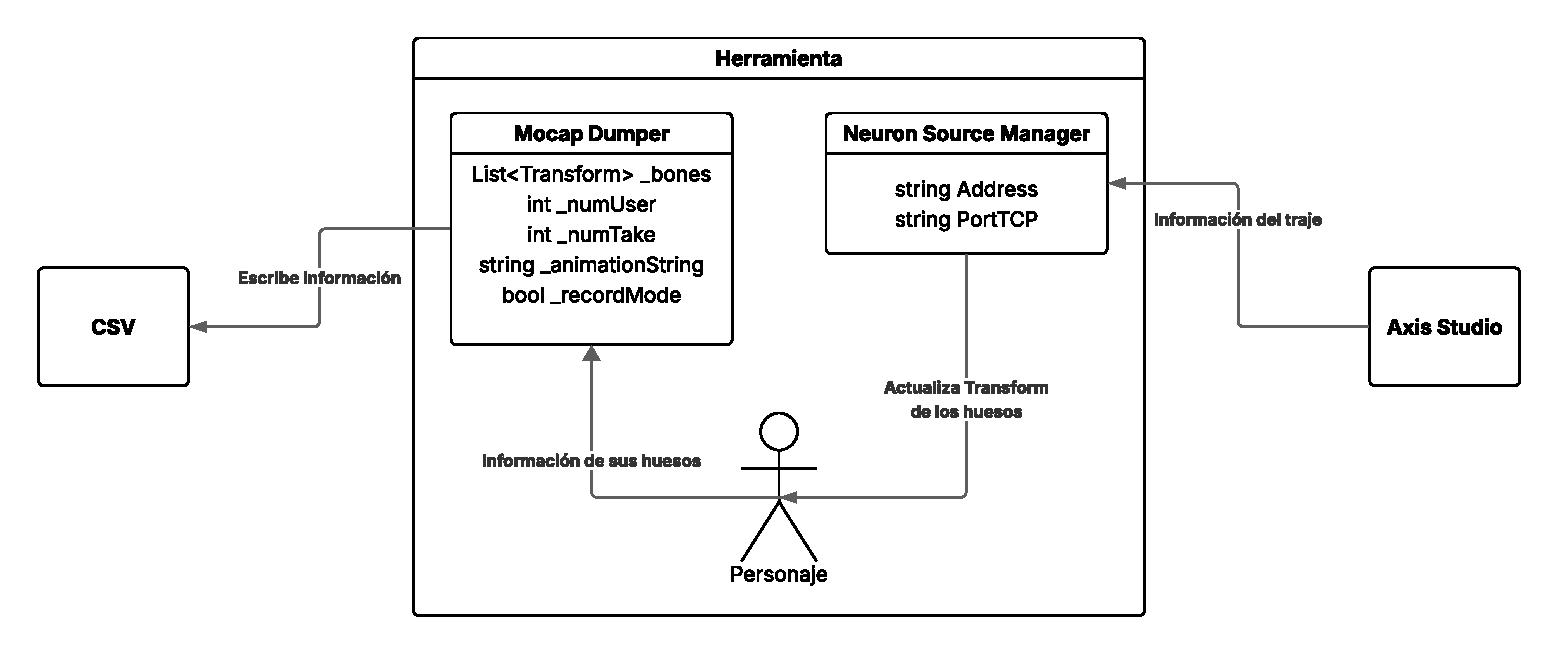
\includegraphics[width=1\textwidth]{Imagenes/Vectorial/MocapDumper.pdf}
	\caption{Diagrama de la conexión entre los distintos componentes de la herramienta, llamada Mocap Dumper}
	\label{fig:MocapDumper}
\end{figure}

\subsection{Recogida de datos}
La recogida de datos consistió en ponerle el traje de captura de movimiento a los usuarios y pedirles que realizasen tres tomas de cada uno de los gestos, a excepción del gesto de baile, ya que de ese gesto había bastantes más datos que el resto.

Para ello se creó un formulario para que los usuarios interesados en ello se apuntasen. En el formulario se explicaba el objetivo de la prueba y se numeraban los datos que iban a ser pedidos en la prueba. Los campos a rellenar eran:

\begin{enumerate}
	%\renewcommand{\theenumi}{\alph{enumi}}
	\item Correo
	\item Aceptar recogida de datos
	\item Posible hueco en un horario, en huecos de una hora de lunes a viernes y de 9:00 a 20:00
\end{enumerate}

Una vez creado el formulario se creó una selección de carteles (figuras \ref{fig:cartel-facultad}, \ref{fig:cartel-redes}, \ref{fig:cartel-pantallas}) el cual se colgó en redes y se colgó en distintas facultades, teniendo como resultado que se apuntasen 75 personas en el formulario.

Lo siguiente era tener un sitio en el que hacer las pruebas. Debido a que las pruebas requerían movimiento era preciso un lugar en el que los usuarios se pudiesen mover sin dificultades y que no estuviese a la vista para preservar la intimidad de los mismos.

Una vez se cerró el formulario, se procedió a hacer un algoritmo que asignara la mayor cantidad de citas posibles dadas las restricciones de tiempo de los usuarios y los días disponibles. El algoritmo\footnote{Enlace al algoritmo: \url{https://github.com/FratosVR/Models/blob/main/citas_generacion_dataset/Scheduler.py}} usa un esquema de ramificación y poda para conseguir la combinación con mayor cantidad de citas disponibles sin tardar más de 10 segundos en procesar las combinaciones válidas.

Finalmente desde el día 14/04/2025 a las 9:00 hasta el día 17/04/2025 a las 19:30 se pudo grabar en el despacho 216 (Sala de grabaciones) de la Facultad de Informática de la Universidad Complutense de Madrid.
De los 75 usuarios apuntados finalmente se presentaron 65, consiguiendo así 975 animaciones en formato CSV, 195 de cada gesto. En la figura \ref{fig:PruebasLidia} se muestra una fotografía de un usuario durante el proceso de calibración.

\begin{figure}[H]
	\centering
	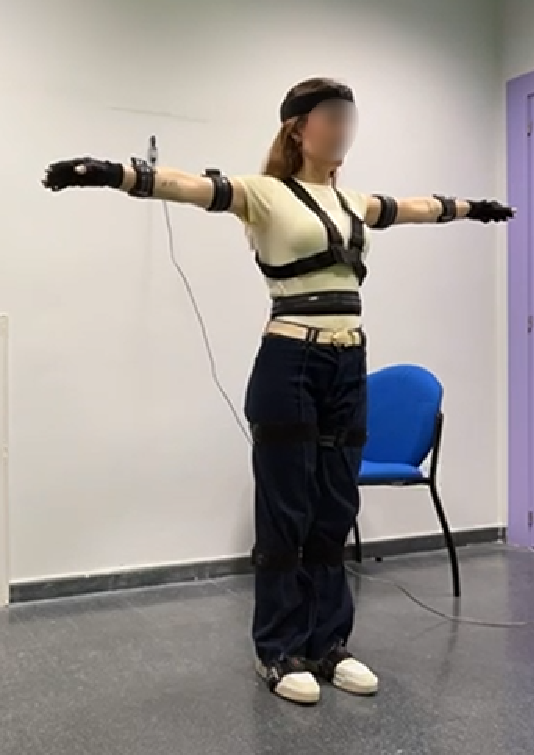
\includegraphics[width=0.5\textwidth]{Imagenes/Vectorial/LidiaPruebasBlurr.pdf}
	\caption{Fotografía de un usuario en las pruebas}
	\label{fig:PruebasLidia}
\end{figure}

A los usuarios no solo se les pidió que realizaran gestos, sino que también se les pidió una serie de información demográfica de manera anónima para saber como de representativa era la muestra. La información pedida fue:

\begin{enumerate}
	%\renewcommand{\theenumi}{\alph{enumi}}
	\item Género
	\item Edad
	\item Nacionalidad
	\item Idiomas hablados
	\item Mano dominante
\end{enumerate}

Estos datos se recogieron con la cuenta de Google de las personas que llevaban el formulario, por lo que no se guardó ningún dato identificable de ningún usuario. En la categoría de género(figura \ref{fig:muestreo-genero}) podemos ver que los datos son un 43.1\% femenino, 50.8\% masculino y 6.2\% no binario. La edad(figura \ref{fig:muestreo-edad}) más común es de 21, con un recuento de un 26.2\% de los encuestados. La nacionalidad (figura \ref{fig:muestreo-nacionalidad}) más común es la española, con un 89.23\% de los encuestados. En la figura \ref{fig:muestreo-idiomas} se puede ver que el idioma más hablado es el español, con un 100\% de los encuestados, seguido de inglés y francés. En la figura \ref{fig:muestreo-mano} se puede ver que el 93.85\% de los encuestados son diestros.

Tras las recogida de datos, se siguió el mismo proceso de estandarización de datos que se usó en el dataset artificial. Antes de estandarizar los datos parecía que se había conseguido eliminar el gran desbalance del dataset hacia los gestos de baile, tras la estandarización de los datos, se vió que las animaciones de baile seguían ganando en cantidad por mucho respecto a las otras. La comparativa se puede ver en las figuras \ref{fig:datos-bruto} y \ref{fig:datos-estandar}.

\begin{figure}[H]
	\centering
	\includegraphics[width=0.7\textwidth]{Imagenes/Bitmap/Distribución_de_animaciones_en_bruto_por_categoria.png}
	\caption{Distribución de los datos brutos}
	\label{fig:datos-bruto}
\end{figure}

\begin{figure}[H]
	\centering
	\includegraphics[width=0.7\textwidth]{Imagenes/Bitmap/Distribución_de_animaciones_adaptadas_por_categoria.png}
	\caption{Distribución de los datos estandarizados}
	\label{fig:datos-estandar}
\end{figure}

El resultado final de todos los datos se puede ver en \cite{csv-pose-animations}. Una vez recogidos y procesados los datos recogidos en las pruebas de usuario se procede al entrenamiento de los distintos modelos para su posterior comparativa.